\label{Chapter4}
 \setstretch{1.5}

\section{Introduction}\label{ch4:sec:Introduction}

%Range (or distance) estimation is important in various localization systems such as global positioning system (GPS)~\cite{Teunissen_GPS_LAMBDA_2006,Teunissen_GPS_1995} and electronic surveying~\cite{Jacobs_ambiguity_resolution_interferometery_1981, anderson1998surveying}. Among various available methods for range estimation, phase of arrival based methods provide the most accurate estimates of the range. However, this method inherits the problem of \emph{phase ambiguity}. Phase ambiguity problem occurs due to an inherent property of the phase that the observed value of the phase is always in the range $[-\pi, \pi)$. This phase ambiguity problem occurs when the unknown range is larger than the wavelength of the signal. This problem is addressed by using multiple different frequencies at the transmitter and observing the phase at each. The range can then be measured within an interval of length equal to the lcm of the wavelengths~\cite{Xiaowei_Li_robust_CRT_2009, W.Wang_closed_form_crt_2010, Li_distance_est_wrapped_phase,Akhlaq_basis_construction_range_est_2015}.
%
%One solution to this problem is based on the Chinese remainder theorem (CRT) when the wavelengths can be scaled to pairwise relatively prime integers. CRT based range estimators are also proposed when the wavelengths can not be scaled to pairwise relatively prime integers~\cite{Oystein_Ore_general_chinese_Remainder_1952, Yuke_new_CRT_1998}. However, it is well known that CRT based range estimators are not robust i.e. a small error in the remainder may produce a large error in the estimated solution. Both approximate and exact techniques for computing the least squares range estimator and related estimators have also been studied by Teunissen~\cite{Teunissen_GPS_1995}, Hassibi and Boyd~\cite{Hassibi_GPS_1998}, Xiaoet~al.~\cite{Li_distance_est_wrapped_phase, Li_coloured_2013} and most recently by Assad~et~al.~\cite{Akhlaq_basis_construction_range_est_2015}.  

%Range (or distance) estimation is an important component of modern technologies such as electronic surveying~\cite{Jacobs_ambiguity_resolution_interferometery_1981, anderson1998surveying} and global positioning~\cite{Teunissen_GPS_LAMBDA_2006,Teunissen_GPS_1995}.  Common methods of range estimation are based upon received signal strength~\cite{Chitte_RSS_Estimation2009, HingCheung_RSSbasedRangeEstimation2012}, time of flight (or time of arrival)~\cite{XinrongLi_TOA_range_estimation2004, Lanzisera_TOA_range_estimation2011}, and phase of arrival~\cite{Jacobs_ambiguity_resolution_interferometery_1981,Towers_frequency_selection_interferometry_2003,Li_distance_est_wrapped_phase}.  This paper focuses on the phase of arrival method which provides the most accurate range estimates in many applications.  Phase of arrival has become the technique of choice in modern high precision surveying and global positioning ~\cite{Odijk-nteger-ambiguity-resolutionPPP, Teunissen_GPS_LAMBDA_2006, Teunissen_GPS_1995}. 
%
%A difficulty with phase of arrival is that only the principal component of the phase can be observed.  This limits the range that can be unambiguously estimated.  One approach to address this problem is to utilise signals of multiple different wavelengths and observe the phase at each.  The range can then be measured within an interval of length equal to the least common multiple of the wavelengths.  Range estimators from such observations have been studied by numerous authors~\cite{Teunissen_GPS_1995,Hassibi_GPS_1998,Towers_frequency_selection_interferometry_2003,Towers:04_generalised_frequency_selection,Li_distance_est_wrapped_phase, Xia2007, XWLi2008,Xiao_multistage_crt_2014}.  Techniques include the beat wavelength method of Towers~et~al.~\cite{Towers_frequency_selection_interferometry_2003,Towers:04_generalised_frequency_selection}, the method of excess fractions~\cite{Falaggis_excess_fractions_2013}, and methods based on the Chinese Remainder Theorem (CRT)~\cite{Oystein_Ore_general_chinese_Remainder_1952,Yuke_new_CRT_1998, Oded_Chinese_remaindering_with_errors_2000, G.Wang_location_and_imaging_2004, Xia_generalised_CRT_2005, Xia2007, XWLi2008, Xiaowei_Li_robust_CRT_2009, W.Wang_closed_form_crt_2010, Xiaowei_Li_location_and_imaging_2011, YangBin_range_estimation_with_CRT_2014, Xiao_multistage_crt_2014}.  Least squares/maximum likelihood and maximum a posteriori estimators of range have been studied by Teunissen~\cite{Teunissen_GPS_1995}, Hassibi and Boyd~\cite{Hassibi_GPS_1998}, and more recently by Li~et~al.~\cite{Li_distance_est_wrapped_phase} and Akhlaq~et~al.~\cite{Akhlaq_basis_construction_range_est_2015}.  A key realisation is that the least squares estimator can be efficient computed by solving a well known integer programming problem, that of computing a \emph{closest point} in a \emph{lattice}~\cite{Agrell2002}.    Teunissen~\cite{Teunissen_GPS_1995} appears to have been the first to have realised this connection.
 


All of the range estimators such as beat wavelength, excess fractions, CRT and least squares either explicitly, or implicitly, make an estimate of so called integer \emph{wrapping variables} related to the whole number of wavelengths that occur over the range.  Given estimates of the wrapping variables, an estimate of the range is typically given by linear regression.  It is expected that accurate estimators of the wrapping variables will also be accurate estimators of the range. Identification of a criterion that guarantees the correctness of these wrapping variables for the least squares range estimator is important because it provides a basis for selecting wavelengths/frequencies to be used for range estimation. In this chapter we first define the \emph{wrapping variables} and then find a condition on the phase measurement errors that guarantees the correctness of these variables. This finding further motivates the search for methods of selecting wavelengths that can maximise the probability of correctness of these wrapping variables, which is the focus of next chapter.

Robust range estimators from erroneous phase measurements (remainders) for CRT based range estimators are proposed in~\cite{Xiaowei_Li_robust_CRT_2009, W.Wang_closed_form_crt_2010} . They derived an upper bound $\taucrt$ such that if all the absolute phase measurement errors are less than $\taucrt$, then the CRT estimator is guaranteed to correctly estimate the wrapping variables. They called $\taucrt$ the \emph{robustness bound}. Their robustness bound holds only if the greatest common divisor (gcd) of all the wavelengths is greater than one and the remaining wavelengths after division by this gcd are co-prime. Recently a robust CRT based range estimator was also proposed in~\cite{Xiao_multistage_crt_2014} for the general case without the constraint used in ~\cite{Xiaowei_Li_robust_CRT_2009, W.Wang_closed_form_crt_2010}. 

In this chapter we derive a similar upper bound $\tauls$ for the least squares range estimator that indicates the superior performance of the least squares range estimator compared to the CRT estimator.  If all absolute phase measurement errors are less than $\tauls$, then the least squares range estimator is guaranteed to correctly estimate the wrapping variables.  The bound is derived from a lattice property called the \emph{inradius}.  We find that  $\tauls > \taucrt$ in many cases.  This corroborates with existing empirical evidence suggesting that the least squares estimator is often more accurate than those estimators based on the CRT~\cite{Akhlaq_basis_construction_range_est_2015}.

The chapter is organised as follows. Section \ref{ch4:sec:phase-and-range-relation} presents the concept of correct wrapping variables.  Section \ref{ch4:sec:robustness-bound} derives our upper bound $\tauls$ for the least squares range estimator based upon the inradius of a lattice.  Section \ref{ch4:sec:sim-results} compares the proposed bound $\tauls$ with the bound $\taucrt$ for the CRT based estimator of Xiao~et~al.~\cite{Xiao_multistage_crt_2014}.  We find that $\tauls > \taucrt$ in many cases.  The results of Monte-Carlo simulations are presented and it is found that the bounds $\tauls$ and $\taucrt$ provide insight about the mean square error of these range estimators.

%**************************************************************************************************************************************************************
%		Section II :  System Model
%**************************************************************************************************************************************************************
\section{Concept of Correct Wrapping Variables}\label{ch4:sec:phase-and-range-relation}
%Suppose that a transmitter sends a sinusoidal signal 
%\[
%s(t)=  \sin (2\pi ft + 2\pi\phi)
%\] 
%with known phase $\phi$. The signal is assumed to propagate by line of sight to a receiver resulting in the signal 
%\[
%y(t) = \alpha s(t - r_0/c) + \omega(t) = \alpha \sin (2\pi ft + 2\pi\theta) +  \omega(t)
%\]
%where $r_0$ is the distance (or range) between the transmitter and the receiver, $c$ is the speed at which the signal propagates, $\alpha$ is the amplitude of the received signal, and $\omega(t)$ represents noise. The phase of the received signal is
%\[
%\theta = \phi - \dfrac{ f }{c}r_0 = \phi - \dfrac{r_0}{\lambda}
%\]
%where $\lambda = c/f$ is the wavelength. In order to estimate the range $r_0$ the receiver first makes an estimate $\hat{\theta} \in [-\tfrac{1}{2}, \tfrac{1}{2})$ of the principal component of the phase $\theta$. The range $r_0$ is related to the phase estimate $\hat{\theta}$ by the phase difference
%\begin{equation*}
%Y = \sfracpart{\phi - \hat{\theta}} = \fracpart{ r_0/\lambda + \Phi },
%\end{equation*}
%where $\Phi$ represents phase noise and $\sfracpart{x} = x - \round{x}$ denotes the \emph{centered} fractional part of $x$, where $\round{x}$ is the  closest integer to $x$ with half integers rounded up. Observe that ranges $r_0$ and $r_0 + k\lambda$ for any integer $k$ result in the same  phase difference $Y$.  For this reason, the range is identifiable from the phase difference only if we assume $r_0$ to lie in some interval of length $\lambda$.  
%%, or more generally, in some set of coset representatives of the quotient group $\reals / \lambda\ints$.  
%A natural choice is the interval $[0, \lambda)$.
%
%This poses a problem if the range $r_0$ is larger than the wavelength $\lambda$.  A common approach to address this problem is to transmit multiple signals at multiple different frequencies and observe the phase at each. In this approach, $N$ phase estimates $\hat{\theta}_1,\ldots,\hat{\theta}_N$ and $N$ phase differences 
%%\begin{equation}\label{eq:Yndefn}
%\begin{equation}\label{eq:Yndefn}
%Y_n = \sfracpart{\phi - \hat{\theta}_n} = \fracpart{ r_0/\lambda_n + \Phi_n}, \qquad n = 1, \dots, N
%%& = \fracpart{ r_0/\lambda_n + X_n} \qquad n = 1,\dots,N 
%%& = r_0/\lambda_n + X_n - z_{0n}
%\end{equation}
%%\end{equation}
%are computed, where $\lambda_n = c/f_n$ is the wavelength of the $n$th signal and $\Phi_1,\dots,\Phi_n$ represent phase noise.  Let $P = \lcm(\lambda_1,\dots,\lambda_N)$ be the least common multiple of the wavelengths.  The least common multiple is the smallest postive integer such that $P/\lambda_1, \dots, P/\lambda_N$ are all integers.  Observe that the ranges $r_0$ and $r_0 + kP$ for any integer $k$ result in the same phase differences $Y_1,\dots,Y_N$ and so $r_0$ can be uniquely identified only within an interval of length $P$.  A natural choice is the interval $[0,P)$.  The least common multiple $P$ is typically much larger than any individual wavelength and so the identifiable range can be considerably enlarged by the use of multiple wavelengths.   If $\lambda_n/\lambda_m$ is irrational for any $n$ and $m$ then the least common multiple $P$ does not exist.  In this paper we assume this is not the case and that a finite least common multiple $P$ does exist.  This is a common assumption in the literature and in practice.  %In what follows we will call the ranges $r_0$ and $r_0 + kP$ as 
%
In this section, we further extend the system model presented in~\ref{ch3:sec:ls-estimator} and define the correct wrapping variables. The understanding of correct wrapping variables is necessary to define the bound $\tauls$ for the least squares range estimator in the next section. Recall that the phase differences can be written in the form 
\begin{align*}
Y_n &=  \fracpart{ r_0/\lambda_n + \Phi_n} =  r_0/\lambda_n + \Phi_n + \zeta_n
\end{align*}
where the integers
\[
\zeta_n = -\round{r_0/\lambda_n + \Phi_n} \qquad n = 1 ,\dots, N 
\]
are called \emph{wrapping variables}. The wrapping variables are related to the number of whole wavelengths that occur over the range $r_0$ between the transmitter and the receiver.  Writing in column vector form
\begin{equation}\label{ch4:eq:Yndefn_vecform}
\ybf = r_0\wbf + \Phibf + \zetabf
\end{equation}
where the column vectors
\[
\ybf = \left(\begin{matrix} Y_1 \\ \vdots \\ Y_N \end{matrix}\right)  \;\; 
\zetabf = \left( \begin{matrix} \zeta_1 \\ \vdots \\ \zeta_N \end{matrix}\right) \;\;
\wbf = \left( \begin{matrix} \frac{1}{\lambda_1} \\ \vdots \\ \frac{1}{\lambda_N} \end{matrix} \right) \;\; 
\Phibf = \left( \begin{matrix} \Phi_1 \\ \vdots \\ \Phi_N \end{matrix} \right) .
\]
%\begin{align*}
%\ybf &= (Y_1,\dots,Y_N)^\prime \in \reals^N, \\
%\zetabf &= (\zeta_1,\dots,\zeta_N)^\prime \in \ints^N, \\
%\wbf &= \left(1/\lambda_1,\dots,1/\lambda_N\right)^\prime \in \reals^N , \\
%\Phibf &=(\Phi_1,\dots,\Phi_N)^\prime \in \reals^N.
%\end{align*}
The $n$th element of the vector $\wbf$ is the reciprocal of the $n$th wavelength, that is, $w_n = 1/\lambda_n$.  Observe $P$ is the smallest positive number such that the vector 
\[
\vbf = P\wbf = (P/\lambda_1, \dots, P/\lambda_N) \in \ints^N,
\]
that is, such that the elements of $\vbf = P\wbf$ are all integers. Equivalently, $P$ is the unique positive real number such that the elements of $\vbf$ are jointly relatively prime, that is, such that 
\[
\gcd(v_1,\dots,v_N) = \gcd(P/\lambda_1, \dots, P/\lambda_N) = 1.
\]
Common range estimators, such as the least squares estimator, those estimators based on the CRT, and the method of excess fractions, operate in two stages. In the first stage, an estimate $\hat{\zetabf}$ of the wrapping variables $\zetabf$ is made. Given $\hat{\zetabf}$, an estimate of the range $r_0$ is typically given by linear regression, that is, 
%\begin{equation}\label{betahatz}
\begin{equation}\label{ch4:eq:rhatlinreg}
\hat{r}  = \frac{(\ybf - \hat{\zetabf})^\prime\wbf}{\wbf^\prime\wbf}
\end{equation}
%\end{equation}
where superscript $^\prime$ indicates the vector or matrix transpose. For any integer $k$, the ranges $r_0$ and $r_0 + kP$ are equivalent and so the range estimates $\hat{r}$ and $\hat{r} + kP$ for any integer $k$ are equivalent.  % To account for this, the least squares range estimator is given by~\cite[Eq.~(6)]{Akhlaq_basis_construction_range_est_2015}
% \begin{equation}\label{hatrangeLS}
% \hat{r}_{\text{LS}}  = \hat{r} - P \floor{\hat{r}/P}.
% \end{equation}
It follows that estimates $\hat{\zetabf}$ and $\hat{\zetabf} + kP\wbf$ of the wrapping variables are equivalent, because
\[
\frac{(\ybf - \hat{\zetabf} + kP\wbf)^\prime\wbf}{\wbf^\prime\wbf} = \hat{r} + kP.
\]
For this reason, the estimated wrapping variables $\hat{\zetabf}$ are to be considered error free (or correct), if $\hat{\zetabf} = \zetabf + kP\wbf$ for some integer $k$.  Because $P$ is the smallest positive integer such that $\vbf = P\wbf \in \ints^N$ this occurs if and only if $\Qbf \hat{\zetabf} = \Qbf \zetabf$ where 
\begin{equation}\label{eq:Qproj}
\Qbf = \Ibf - \frac{\wbf\wbf^\prime}{\wbf^\prime\wbf} = \Ibf - \frac{\vbf\vbf^\prime}{\vbf^\prime\vbf}
\end{equation}
is the $N \times N$ orthogonal projection matrix onto the $N-1$ dimensional subspace orthogonal to $\wbf$ and $\Ibf$ is the $N\times N$ identity matrix.  In what follows, estimates $\hat{\zetabf}$ of the wrapping variables $\zetabf$ are said to be \emph{correct} if $\Qbf \hat{\zetabf} = \Qbf \zetabf$.

Xiao~et~al.~\cite{Xiao_multistage_crt_2014} derived an upper bound 
\begin{equation}\label{eq:crt-upper-bound}
\tau_{_{CRT}} =  \frac{1}{4c \lambda_{\max}}\min_{1\leq i \leq N}  \min_{1\leq j \neq i \leq N} \gcd (c\lambda_i, c\lambda_j)
\end{equation} 
such that if the absolute values of the phase noise are less than $\taucrt$, then the CRT estimator is guaranteed to correctly estimate the wrapping variables.  That is, if  $\abs{\Phi_n} < \taucrt$ for all $n = 1, \dots, N$, then $\Qbf \hat{\zetabf} = \Qbf\zetabf$.  The value $\lambda_{\text{max}} = \max_n \lambda_n$ is the maximum wavelength and $c$ is a positive real number such the scaled wavelengths $c \lambda_1, \dots, c \lambda_N$ are all integers.  The existance of $c$ is guaranteed by the fact that the wavelengths are assumed to be rationally related, that is, $\lambda_n/\lambda_k$ is rational for all $n$ and $k$.

In the next section we will find a similar upper bound $\tauls$ for the least squares range estimator.  It is shown in \Sec{ch3:sec:range-estim-clos-1}, that the least squares estimator $\hat{\zetabf} \in \ints^N$ of the wrapping variables minimises the quadratic form
\begin{equation}\label{eq:hatz}
\| \Qbf\ybf - \Qbf\zbf \|^2 \qquad \text{over $\zbf \in \ints^N$},
\end{equation}
where $\|\cdot\|$ indicates the Euclidean norm of a vector.  Given $\hat{\zetabf}$, the least square range estimator $\hat{r}$ is then given by~\ref{ch4:eq:rhatlinreg}.  It is shown in \Sec{ch3:sec:range-estim-clos-1} how the quadratic form~\ref{ch3:eq:hatz} can be minimised over $\ints^N$ by computing a closest point in a \emph{lattice}.  We will derive the bound $\tauls$ by using a property of this lattice from \Sec{sec:ch2-lattice-theory} called the \emph{inradius}. 

%It is shown in~\cite{Akhlaq_basis_construction_range_est_2015}, that the least squares estimate $\hat{\zetabf} \in \ints^N$ of the wrapping variables minimises the quadratic form
%\begin{equation}\label{eq:hatz}
%\| \Qbf\ybf - \Qbf\zbf \|^2 \qquad \text{over $\zbf \in \ints^N$},
%\end{equation}
%where $\|\cdot\|$ indicates the Euclidean norm of a vector.  It is shown in~\cite{Akhlaq_basis_construction_range_est_2015} how this quadratic form can be minimised over $\ints^N$ by computing a closest point in a lattice.  We will derive the bound $\tauls$ by studying a property of this lattice called the \emph{inradius}.  We first require some introductory concepts from lattice theory.

% If we denote this subspace by $H$ then by~\cite[Corollary 1]{Akhlaq_basis_construction_range_est_2015} the set $\Lambda = \ints^N \cap H$ and the set $\Lambda^* = \{ \Qbf \zbf \mid \zbf \in \ints^N \}$.  We see that the problem of minimising~\eqref{eq:hatz} is precisely that of finding a closest lattice point in $\Lambda^*$ to $\Qbf\ybf \in \reals^N$.  
% A solution to~\eqref{eq:hatz} is provided in~\cite{Akhlaq_basis_construction_range_est_2015} by solving a problem from computational number theory called the closest lattice point~\cite{Agrell2002}. Given estimates $\hat{\zetabf}$ of the wrapping variables  the least squares estimate of $r_0$ is given as~\cite{Akhlaq_basis_construction_range_est_2015}


%**************************************************************************************************************************************************************
%		Section III :  Lattice theory
%**************************************************************************************************************************************************************
%\section{Lattice theory}\label{ch4:sec:lattice-theory}
%
%Let $\mathbf{b}_1,....,\mathbf{b}_n$ be linearly independent vectors from $m$-dimensional Euclidean space $\reals^m$ with $m\geq n$.  The set of vectors
%\[
%\Lambda = \{ u_1\bbf_1 + \dots + u_n \bbf_n \mid u_1,\dots,u_n \in \ints \}
%\]
%is called an $n$-dimensional \term{lattice}.  The elements of $\Lambda$ are called \term{lattice points} or \term{lattice vectors}. 
%The vectors $\bbf_1,\dots,\bbf_n$ form a \emph{basis} for the lattice $\Lambda$.  We can equivalently write
%\[
%\Lambda=\{ \Bbf\ubf \mid \ubf \in \ints^n \}
%\]
%where $\Bbf$ is the $m\times n$ matrix with columns $\bbf_1,\dots,\bbf_n$. The matrix $\Bbf$ is called a \term{basis} or \term{generator} for $\Lambda$. When $m = n$ the lattice is said to be \term{full rank}. When $m > n$ the lattice points lie in the $n$-dimensional subspace of $\reals^m$ spanned by $\bbf_1,\dots,\bbf_n$.  %The set of integers $\ints^n$ is called the \term{integer lattice} with the $n \times n$ identity matrix $\bf{I}$ as a basis.
%
%%The parallelepiped formed by basis vectors $\bbf_1,\dots,\bbf_n$ is called a \term{fundamental parallelepiped} of the lattice $\Lambda$.  A fundamental parallelepiped has $n$-dimensional volume $\sqrt{\det \Bbf^\prime\Bbf }$ where superscript $^\prime$ denotes the vector or matrix transpose.  This quantity is also called the determinant of the lattice and is denoted by $\det\Lambda$.  
%The (closed) \term{Voronoi cell}, denoted $\vor\Lambda$, of an $n$-dimensional lattice $\Lambda$ in $\reals^m$ is the subset of $\reals^m$ containing all points nearer or of equal distance (here with respect to the Euclidean norm) to the lattice point at the origin than to any other lattice point (Figure~\ref{fig:bound_dmin}).  % Equivalently, the Voronoi cell can be defined as the intersection of the half spaces 
%% \begin{align*}
%% H_{\wbf} &= \{\xbf \in \reals^n \mid \|\xbf\| \leq \|\xbf - \wbf\| \} \\
%% &= \{\xbf \in \reals^n \mid \dotprod{\xbf}{\wbf} \leq \tfrac{1}{2}\dotprod{\wbf}{\wbf} \}
%% \end{align*}
%% for all $\wbf \in \Lambda \backslash  \{\zerobf\}$ where $\Lambda \backslash  \{\zerobf\}$ denotes the set of lattice points not equal to the origin $\zerobf$.
%The Voronoi cell $\vor\Lambda$ tesselates $\reals^N$ in the sense that
%\[
%\reals^N = \bigcup_{\xbf \in \Lambda} (\vor\Lambda + \tbf)
%\]
%and $\vor\Lambda$ and a translate $\vor\Lambda + \tbf$ by a lattice point $\tbf \in \Lambda\backslash  \{\zerobf\}$ intersect at most on the boundary of $\vor\Lambda$.  The set $\Lambda \backslash  \{\zerobf\}$ denotes those lattice points from $\Lambda$ not equal to the origin $\zerobf$.  In particular, if $\interior\Lambda$ denotes the interior of the Voronoi cell, then the intersection of $\interior\Lambda$ and $\vor \Lambda + \tbf$ is empty for all $\tbf \in \Lambda \backslash  \{\zerobf\}$.  % Equivalently, if $\tbf \in \Lambda$, $\wbf \in \vor\Lambda$, and $\ybf \int\Lambda$, and
%% \[
%% \]
%This leads to the following simple property that we will find useful.
%
%\begin{remark}\label{remarksimpleintvor}
%If $\tbf \in \Lambda$, $\ubf \in \vor\Lambda$, $\vbf \in \interior\Lambda$, and $\ubf = \vbf + \tbf$, then $\tbf = \zerobf$.
%\end{remark}
%
%%Let $\Lambda$ be an $n$-dimensional lattice and let $H$ be the $n$-dimensional subspace spanned by its lattice points. The \term{dual lattice} of $\Lambda$, denoted $\Lambda^*$, contains those points from $H$ that have integer inner product with all points from $\Lambda$, that is,
%%\[
%%\Lambda^* = \{ \xbf  \in H \mid \xbf^\prime \ybf \in \ints \text{ for all } \ybf \in \Lambda \}.
%%\] 
%% 
%Given a vector $\ybf \in \reals^m$, a problem of interest is to find a lattice point $\xbf \in \Lambda$ such that the squared Euclidean norm
%\[
%\| \ybf - \xbf \|^2 = \sum_{i=1}^m (y_i - x_i)^2 
%\]  
%is minimised.  This is called the \term{closest lattice point problem} (or \term{closest vector problem}) and a solution is called a \term{closest lattice point} (or simply \term{closest point}) to $\ybf$ \cite{Agrell2002,McKilliam2009CoxeterLattices,MicciancioVoulgaris_deterministic_jv_2013,McKilliam_closest_point_lattice_first_kind_2014}.  The closest lattice point problem and the Voronoi cell are related in that $\xbf\in\Lambda$ is a closest point to $\ybf$ if and only if $\ybf - \xbf \in \vor\Lambda$. 
%
%A \emph{short vector} in a lattice $\Lambda$ is a lattice point of minimum nonzero Euclidean length, that is, a lattice point of length
%\[
%\dmin =  \min_{\xbf \in \Lambda \backslash \{ \zerobf \} } \| \xbf \|^2.
%\]   
%The length $\dmin$ of a short vector is the smallest distance between any two lattice points.  The \emph{inradius} or \emph{packing radius} $\rho = \dmin/2$ is the length of a point on the boundary of the Voronoi cell that is closest to the origin (Figure~\ref{fig:bound_dmin}).  Equivalently, the inradius is the radius of the largest sphere that fits inside the Voronoi cell.  It is also the radius of the largest sphere that can be centered at each lattice point such that no two spheres intersect.  Such an arrangement of spheres is called a \emph{sphere packing} (Figure~\ref{fig:bound_dmin}).
%
%% For a given lattice $\Lambda$ with generator matrix $\mathbf{B}$, the minimum distance of the lattice or the length shortest lattice vector $d_{\min}$ is defined as 
%  
%%  \[
%%  d_{\min} = \underset{\zbf \in \mathbf{\ints}^n , \zbf\neq 0}{\operatorname{min}} \|\mathbf{Bz} \|. 
%%  \]
%%  $d_{\min}$ is the length of the shortest lattice vector other than origin i.e. it is the distance between the origin and its closest lattice point as shown in Figure~\ref{fig:bound_dmin}. The inradius of a lattice is equal to the half of the length of the shortest lattice vector i.e. $\frac{d_{\min}}{2}$.
% 
%\begin{figure}[t]
%\begin{center} 
%%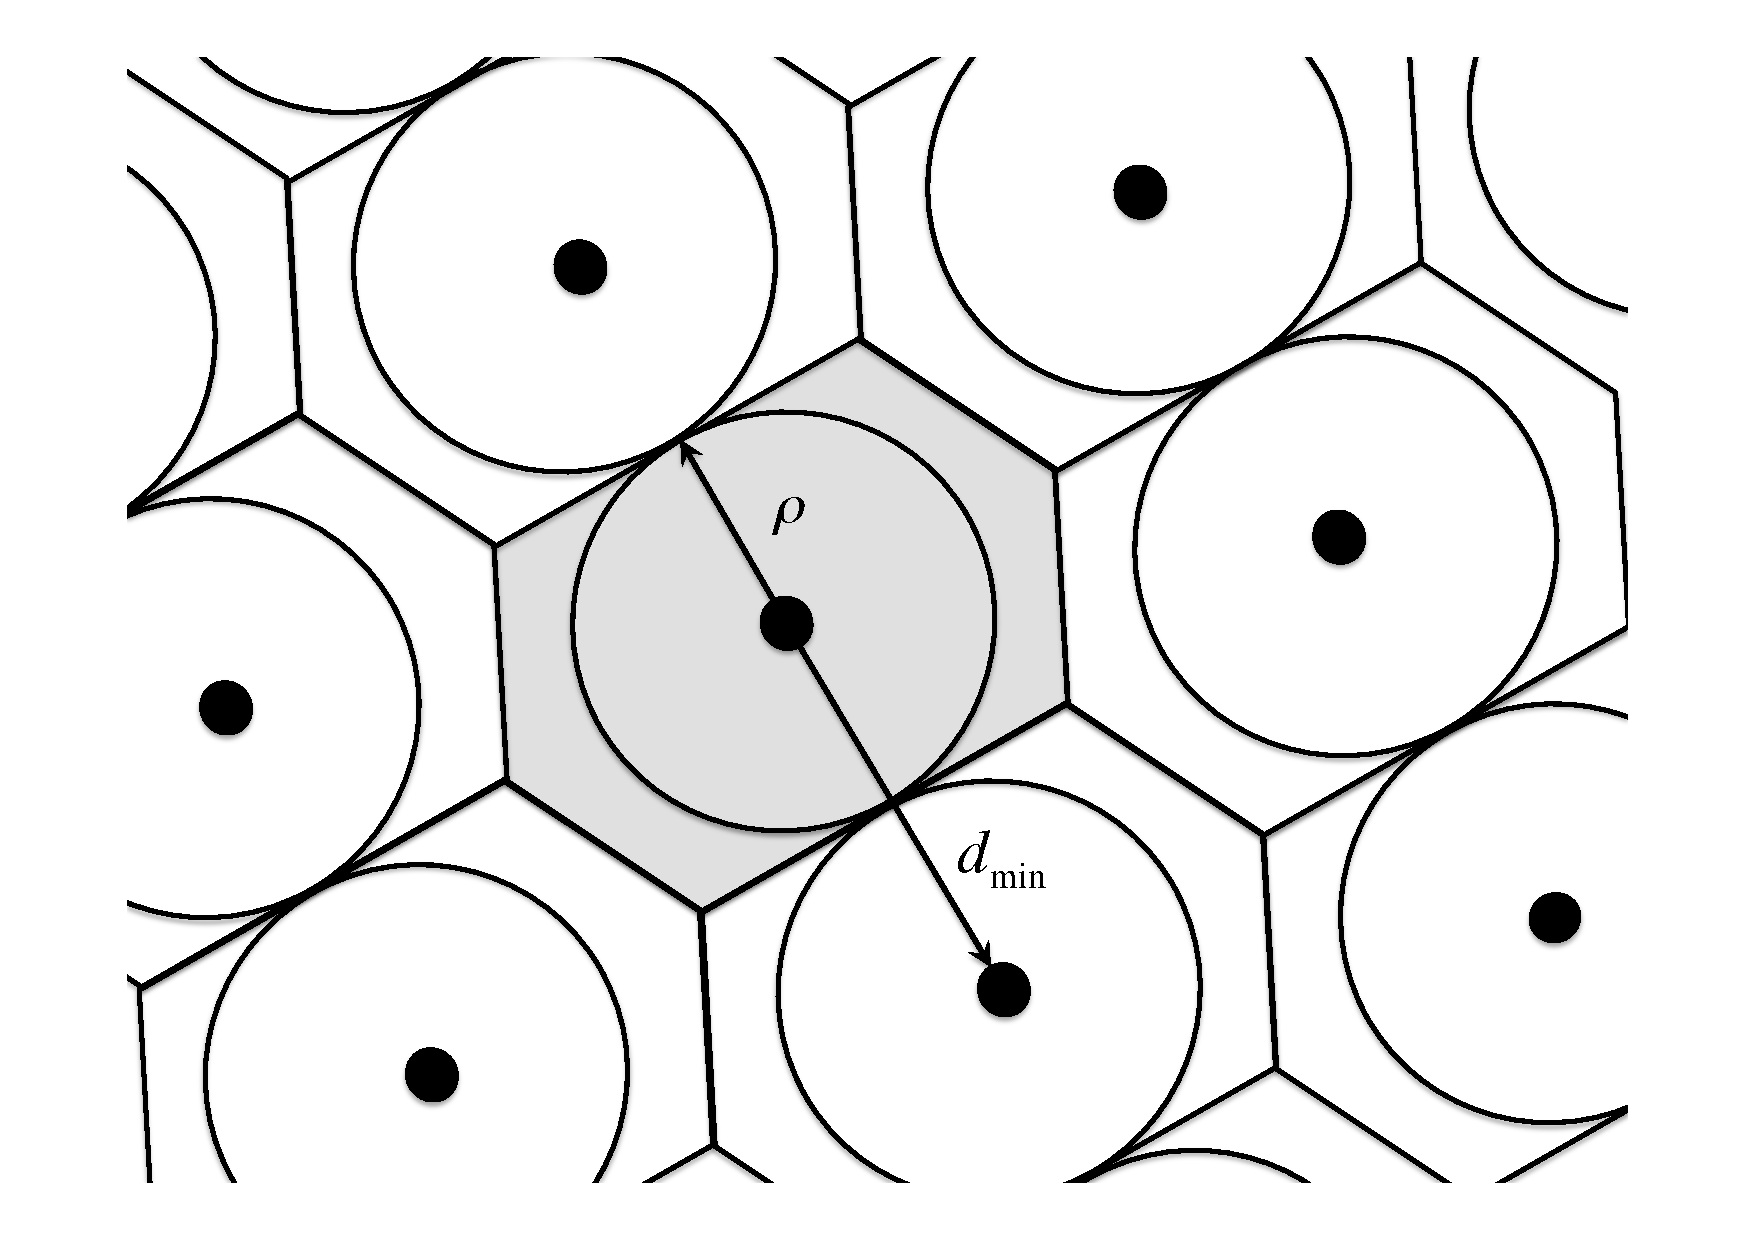
\includegraphics[scale=0.30]{figs/bound_dmin.pdf} 
%%\caption{The length of a short vector $\dmin$ and inradius $\rho = \dmin/2$ of the 2-dimensional lattice. This lattice has two short vectors. The shaded region shows the Voronoi cell of the lattice. The circles exhibit a sphere packing.}
%\includegraphics{chapters/ch4/Figs/latticefigures-1.mps}
%\caption{The length of a short vector $\dmin$ and inradius $\rho = \dmin/2$ of the 2-dimensional lattice with basis $\bbf_1 = [3,0.6]^\prime, \bbf_2 = [0.6,3]^\prime$. This lattice has four short vectors.  The shaded region shows the Voronoi cell of the lattice.  The circles exibit a sphere packing.}
%\label{fig:bound_dmin}
%\end{center}  
%\end{figure} 
%  
%**************************************************************************************************************************************************************
%		Section IV : Criterion for robust range estimation
%**************************************************************************************************************************************************************
\section{Bound for the least squares range estimator}\label{ch4:sec:robustness-bound}

Recall that the least squares estimate $\hat{\zetabf}$ of the wrapping variables $\zetabf$ minimises the quadratic form $\|\Qbf \ybf - \Qbf \zbf\|^2$ over $\zbf \in \ints^N$, that is,
\[
\|\Qbf \ybf - \Qbf \hat{\zetabf}\|^2 = \min_{\zbf \in \ints^N} \|\Qbf \ybf - \Qbf \zbf\|^2.
\]
It is shown in~\refchapter{Chapter3} that the set
\[
\Lambda^* = \{ \Qbf\zbf \mid \zbf \in \ints^N  \}
\]
is an $N-1$ dimesional lattice.  Thus, $\Qbf\hat{\zetabf}$ is a lattice point in $\Lambda^*$ and, because 
\begin{align*}
\|\Qbf \ybf - \Qbf \hat{\zetabf}\|^2 &= \min_{\zbf \in \ints^N} \|\Qbf \ybf -  \Qbf \zbf\|^2 \\
&= \min_{\xbf \in \Lambda^*} \|\Qbf \ybf - \xbf\|^2,
\end{align*}
it follows that $\Qbf \hat{\zetabf}$ is a closest lattice point to $\Qbf\ybf$.  Because of this, $\Qbf \ybf - \Qbf \hat{\zetabf}$ is an element of the Voronoi cell of the lattice $\Lambda^*$, that is,
\[
\Qbf \ybf - \Qbf \hat{\zetabf} = \Qbf ( \ybf -  \hat{\zetabf} ) \in \vor \Lambda^*.
\]
Observe from~\ref{ch4:eq:Yndefn_vecform} that
\begin{align*}
\Qbf (\ybf - \hat{\zetabf}) &= \Qbf (r_0\wbf + \Phibf + \zetabf - \hat{\zetabf}) \\
&= \Qbf \Phibf - \Qbf(\zetabf - \hat{\zetabf}).
\end{align*}
Suppose that the projection of the phase noise $\Qbf \Phibf$ is in the interior of the Voronoi cell $\interior \Lambda$.  Then, it follows from Remark~\ref{remarksimpleintvor} of~\refchapter{Chapter2}, with $\tbf = \Qbf(\zetabf - \hat{\zetabf})$, $\ubf = \Qbf (\ybf - \hat{\zetabf})$, and $\vbf = \Qbf \Phibf$, that $\Qbf(\zetabf - \hat{\zetabf}) = \zerobf$ or equivalently $\Qbf\zetabf =\Qbf\hat{\zetabf}$.

We have found that the least squares estimate $\hat{\zetabf}$ of the wrapping variables is correct whenever the projection of the phase noise $\Phibf$ orthogonal to $\wbf$ is contained in the interior of the Voronoi cell, that is, if $\Qbf \Phibf \in \interior \Lambda$, then $\Qbf \hat{\zetabf} = \Qbf \zetabf$.  Let $\rho = \dmin/2$ be the inradius of the lattice $\Lambda^*$.  If $\|\Qbf \Phibf\| < \rho$ then $\Qbf \Phibf \in \interior \Lambda$ and so $\Qbf \hat{\zetabf} = \Qbf \zetabf$.  Becasue $\Qbf$ is an orthogonal projection matrix $\|\Phibf\| \geq \|\Qbf\Phibf\|$ and so 
\begin{align*}
&\|\Phibf\| < \rho \\
\implies &\|\Qbf\Phibf\| < \rho \\
\implies &\Qbf \hat{\zetabf} = \Qbf \zetabf,
\end{align*}
that is, the least squares estimate $\hat{\zetabf}$ of the wrapping variables is correct whenever the Euclidean norm of the phase noise is less than the inradius $\rho$ of the lattice $\Lambda^*$.  The inradius $\rho$ depends upon the lattice $\Lambda^*$ which in turn depends upon the wavelengths.  This naturally leads to the question of whether it is possible to select wavelengths that maximise the inradius.  This is an interesting and nontrivial problem that we intend to investigate in future research.


% For the least squares estimator we say that the wrapping variable $\hat{\zetabf}$ are correct if $\Qbf \zetabf = \Qbf \hat{\zetabf}$.  To see why this definition is valid, observe that $\hat{\zetabf} = \zetabf + a \wbf$ where $a$ is such that $a\wbf \in \ints^{N}$.  Because the least common multiple $P$ is the smallest positive number such that $P\wbf$ contains only integers, it follows that $a = kP$ for some integer $k$.  Now, the regression estimator of the range satisfies
% \[
% \hat{r} = \frac{(\ybf - \hat{\zetabf})^\prime\wbf}{\wbf^\prime\wbf} = \frac{(\ybf - \zetabf + kP\wbf)^\prime\wbf}{\wbf^\prime\wbf} = \frac{(\ybf - \zetabf)^\prime\wbf}{\wbf^\prime\wbf} + kP
% \]
% and, from~\eqref{hatrangeLS}, the least square estimator of the range is
% \[
% \hat{r}_{\text{LS}}  = \frac{(\ybf - \hat{\zetabf})^\prime\wbf}{\wbf^\prime\wbf} - P \floor{\hat{r}} = 
% \]

%In this section we provide a bound on phase errors to robustly estimate the wrapping variables, and hence the range, from multiple noisy phase observations. %\subsection{Estimating the wrapping variables}
%It can be observed from~\eqref{eq:Yndefn} that 
%\[
%\fracpart{Y_n - r/\lambda_n}^2 = (Y_n - r/\lambda_n - z_n)^2
%\]
%where $z_n$ $(n=1,\ldots, N)$ are often called \emph{wrapping variables}. These wrapping variables are related to the number of whole wavelengths that occur over the range $r_0$ between the transmitter and the receiver.
%In \cite{Akhlaq_basis_construction_range_est_2015}, we showed how the least squares range estimator $\hat{r}$  from \eqref{eq:hatdininterval} can be efficiently computed by computing a closest point in a lattice of dimension $N-1$. The wrapping variables $\zbf = [z_1,\ldots,z_n]'$ are obtained by minimising the function~\cite{Akhlaq_basis_construction_range_est_2015}
%\[
%F(\zbf) = \| \Qbf\ybf - \Qbf\zbf \|^2
%\]
%where $\Qbf = \Ibf - \wbf\wbf^\prime/\|\wbf\|^2$ is the orthogonal projection matrix onto the $N-1$ dimensional subspace orthogonal to $\wbf$. If we denote this subspace by $H$ then by~\cite[Corollary 1]{Akhlaq_basis_construction_range_est_2015} the set $\Lambda = \ints^N \cap H$ is an $N-1$ dimensional lattice with determinant $\|\wbf\|$ and dual lattice $\Lambda^* = \{ \Qbf \zbf \mid \zbf \in \ints^N \}$.  We see that the problem of minimising $F_2(\zbf)$ is precisely that of finding a closest lattice point in $\Lambda^*$ to $\Qbf\ybf \in \reals^N$.  
%
%Suppose we find $\hat{\xbf} \in \Lambda^*$ closest to $\Qbf \ybf$ and a corresponding $\hat{\zbf} \in \ints^N$ such that $\hat{\xbf} = \Qbf\hat{\zbf}$.  Then $\hat{\zbf}$ minimises $F_2$ and $\hat{\beta}(\hat{\zbf})$ minimises $F$.  The least squares range estimator in the interval $[0,P)$ is then
%\begin{equation}\label{eq:leastsquaresrangehatz}
%\hat{r} = P\big(\hat{\beta}(\hat{\zbf}) - \sfloor{\hat{\beta}(\hat{\zbf})}\big). %= P\left(\frac{(\ybf - \hat{\zbf})^\prime\wbf}{\wbf^\prime\wbf} - \floor{\frac{(\ybf - \hat{\zbf})^\prime\wbf}{\wbf^\prime\wbf}} \right)
%\end{equation}
%Let $V$ denotes the interior of the Voronoi cell $\vor\Lambda^*$. Note that $\hat{\zetabf}$ is a minimiser of $\| \Qbf (\ybf - \zbf) \|$ over $\zbf \in \ints^N$. %We say that the estimator is robust when $\hat{\zetabf}=\zetabf$.
% wrapping variables $\hat{\zbf}$ are ``correct'' if $\Qbf \hat{\zbf} = \Qbf \zbf_0$, that is, the estimates of the wrapping variables $\hat{\zbf}$ when the true range $r_0$ is known i.e. $\hat{\zbf}=\zbf_0$ . From~\eqref{eq:Yndefn}, we have
%\begin{align*}
%Y_n &= \fracpart{ r_0/\lambda_n + X_n} = \fracpart{ \beta_0 w_n + X_n} \\ %r_0/\lambda_n + X_n + z_{0n}\\
%&= \beta_0 w_n + X_n + z_{0n}
%\end{align*}
%where $r_0= P\beta_0 $, $w_n = P/\lambda_n$ and
%\[
%z_{0n} = -\round{\beta_0 w_n + X_n} = -\round{\dfrac{r_0}{\lambda_n} + X_n} 
%\]
% is the $n$th element of the vector $\zbf_0$. Observe that $\ybf - \zbf_0 = \beta_0 \wbf + \xbf$ because
%\[
%Y_n - z_{0n} = \fracpart{\beta_0 w_n +  X_n} + \round{\beta_0 w_n +  X_n} = \beta_0 w_n +  X_n
%\]
%where $\xbf = (X_1,\dots,X_N)^\prime$ is the column vector containing the phase noise. 
% Equivalently, $\Qbf (\ybf - \hat{\zetabf})$ is contained in the Voronoi cell $\vor\Lambda^*$. Now
% So  $\Qbf\zetabf = \Qbf\hat{\zetabf}$ only if $\Qbf\Phibf \in V$. In the following we provide an upper bound $\tau_{_{LS}}$ on phase errors such that $\Qbf\Phi$ is in $V$. This bound is based on the inradius of the lattice $\Lambda^*$. %It will be shown in the simulations results that the robustness bound obtained using the in-radius provides a better bound.

%\subsection{Upper bound $\tau_{_{LS}}$ on phase errors}

% Let $d_{\min}$ be the length of the shortest lattice vector in $\Lambda^*$ i.e. it is the distance between the origin and the closest lattice point in $\Lambda^*$. Then a sphere of radius $\rho = \tfrac{d_{\min}}{2}$ centred at the origin is the largest ball that lies inside $\vor\Lambda^*$ as shown in Figure \ref{fig:bound_dmin}. The radius $\rho$ is called the inradius of the Voronoi cell. Note that $\Qbf\hat{\zetabf} = \Qbf\zetabf$ when $\Qbf\Phi \in \vor\Lambda^*$, that is, $\Qbf\Phi$ lies inside a sphere of radius $\rho$ centred at the origin i.e.
%  \begin{equation}\label{eq-lowerbound-as-QPhi}
% % P_r(\Lambda,\sigma^2) \geq Pr(\|\xbf \| < \rho),
% \|\Qbf\Phi \| < \rho.
% \end{equation}
% As $\Qbf$ is the projection matrix it implies that $\| \Qbf\Phi \| \leq \| \Phi \|$. Therefore \eqref{eq-lowerbound-as-QPhi} is still satisfied if
%  \begin{equation}\label{eq-lowerbound-as-Phi}
% \|\Phi \|^2 < \rho^2.
% \end{equation}
% %Robust estimation requires that the length of the noise vector $\| \xbf \|$ is less than the inradius $\rho$ of the Voronoi cell, i.e.
% From~\eqref{eq-lowerbound-as-Phi}
We now define our bound $\tauls$ for the least squares range estimator.  Observe that if
\begin{equation}\label{eq:robust-reconstruction_criterion}
\abs{\Phi_n} < \frac{\rho}{\sqrt{N}} = \tau_{_{LS}}
\end{equation}
for all $n = 1, \ldots, N$, then
\[
\|\Phibf \|^2 = \sum_{n = 1}^N \Phi_n^2 < \rho^2.
\]
It follows that the least squares estimate of the wrapping variables is correct whenever the absolute value of the phase noise $\abs{\Phi_n} < \tauls = \rho/\sqrt{N}$ for all $n = 1, \dots, N$.

We now compare the bound $\tauls$ with the bound $\taucrt$ from~\ref{eq:crt-upper-bound} derived by Xiao~et~al.~\cite{Xiao_multistage_crt_2014}.  We will find that $\tauls > \taucrt$ is many cases.  We will also find that the bounds $\tauls$ and $\taucrt$ provide insight about the mean square error of these range estimators.

 % still holds and $\Qbf\hat{\zetabf} = \Qbf\zetabf$. Therefore, if each element $\Phi_n$ of the phase noise $\Phi$ is less than  $\tau_{_{LS}} = \frac{\rho}{\sqrt{N}}$ then $\Qbf\hat{\zetabf} = \Qbf\zetabf$. Although~\eqref{eq-lowerbound-as-Phi} provides a better bound than~\eqref{eq:robust-reconstruction_criterion}, however, in this paper we focus on~\eqref{eq:robust-reconstruction_criterion} for its comparison with the bound $\tau_{_{CRT}}$ for the CRT based estimator. Based on our simulation results in the next section we conjecture that this value of $\tau_{_{LS}}$ can be used as a good performance metric for the least squares range estimator.


%Based on our simulation results in the next section we conjecture that the bound $\tau_{_{LS}}$ on the phase errors for the least squares range estimator is larger than or equal the boud $\tau_{_{CRT}}$ for the CRT range estimator. Furthermore the comparison of both the bounds provides us useful information about the comparative performance of the individual range estimators.
%**************************************************************************************************************************************************************
%		Section V : Simulation Results
%**************************************************************************************************************************************************************
\section{Numerical Results}\label{ch4:sec:sim-results}

%%%%%%%%%%%%%%%%%%%%%%%%%%%%%%%%%%%%%%%%%%%%%%%%%%%%%%%%%%%%%%%%%%%%%
\begin{figure}

  \centering 
  \begin{tikzpicture}
    \selectcolormodel{gray} 
    \begin{axis}[
    	legend columns=-1,
	legend entries={$(x+0)^k$;,$(x+1)^k$;,$(x+2)^k$;,$(x+3)^k$},
	legend to name=named,
    font=\footnotesize,xmode=log,ymode=log,height=10cm,width=12cm,ymin=1e-1,ymax=1.2e0,ylabel={$P_c$},ylabel style={at={(-0.085,0.55)}},xlabel style={at={(0.53,-0.05)}}, legend style={draw=none, fill=none, at={(1,1)}, legend pos=south east,legend cell align=left, inner xsep = 1pt, inner ysep = 1pt, nodes = {inner sep=0.05pt, text depth = 0.05cm}},xmin=1e-4,xmax=2e-2,xlabel={$\sigma^2$} ]
	% \addplot[dashed] table {Chapter5/Figs/LeastSquaresA};
	\addplot[mark=*,only marks,mark options={scale= 0.5}] table {chapters/ch4/Figs/ProbLS_A_Uniform};
        \addplot[mark=o,only marks,mark options={scale= 1}] table {chapters/ch4/Figs/ProbCRT_A_Uniform};
        \addplot[mark=x,only marks,mark options={scale= 1}] table {chapters/ch4/Figs/ProbEF_A_Uniform};
        \addplot[mark=none] coordinates {(1.2e-3,1e-3) (1.2e-3,4e0)};
        \addplot[dashed, mark=none] coordinates {(4.69e-4,1e-3) (4.69e-4,4e0)};
  %      	\legend{LS A, CRT A, EF A, Bound LS A, Bound CRT A}
   \end{axis}  
  \end{tikzpicture}   
 %\caption{Probability of correct estimation of the wrapping variables and robustness bounds for the least squares range estimator and the CRT range estimator of Xiao~et~al.~\cite{Xiao_multistage_crt_2014} with $N=3$ wavelenths.}\label{fig:leastsquares_Pc_CRT_N3}   
\\ \vspace{0.1cm}

  \begin{tikzpicture}
    \selectcolormodel{gray} 
    \begin{axis}[font=\footnotesize,xmode=log,ymode=log,height=10cm,width=12cm,ymin=7e-1,ymax=4e5,ylabel={MSE},ylabel style={at={(-0.09,0.55)}},xlabel style={at={(0.53,-0.05)}}, legend style={draw=none, fill=none, at={(1,1)}, legend pos=south east, legend cell align=left, inner xsep = 1pt, inner ysep = 1pt, nodes = {inner sep=0.05pt, text depth = 0.05cm}},xmin=1e-4,xmax=2e-2,xlabel={$\sigma^2$}]
	% \addplot[dashed] table {Chapter5/Figs/LeastSquaresA};
	\addplot[mark=*,only marks,mark options={scale= 0.5}] table {chapters/ch4/Figs/MSELS_A_Uniform};
        \addplot[mark=o,only marks,mark options={scale= 1}] table {chapters/ch4/Figs/MSECRT_A_Uniform};
         \addplot[mark=x,only marks,mark options={scale= 1}] table {chapters/ch4/Figs/MSEEF_A_Uniform};
        \addplot[mark=none] coordinates {(1.2e-3,7e-1) (1.2e-3,4e5)};
        \addplot[dashed, mark=none] coordinates {(4.69e-4,7e-1) (4.69e-4,4e5)};
      	\legend{LS A, CRT A, EF A, Bound LS A, Bound CRT A}
   \end{axis}  
  \end{tikzpicture}   
 %\caption{Sample mean square error of the least squares range estimator and the range estimator based on the single stage CRT algorithms of Xiao~et~al.~\cite{Xiao_multistage_crt_2014} with $N=4$ wavelenths.}\label{fig:leastsquares_MSE_CRT_N3}    

\caption{Probability of correct estimation of wrapping variables $P_c$ (top), sample mean square error (MSE) (bottom), and bounds on variance with wavelengths $A $.} \label{fig:eastsquares_CRT-1}  
\end{figure}

%%%%%%%%%%%%%%%%%%%%%%%%%%%%%%%%%%%%%%%%%%%%%%%%%%%%%%%%%%%%%%%%%%%%%
%%%%%%%%%%%%%%%%%%%%%%%%%%%%%%%%%%%%%%%%%%%%%%%%%%%%%%%%%%%%%%%%%%%%%
\begin{figure}
\hspace{2ex}
  \centering 
  \begin{tikzpicture}
    \selectcolormodel{gray} 
    \begin{axis}[font=\footnotesize,xmode=log,ymode=log,height=10cm,width=12cm,ymin=1e-1,ymax=1.2e0,ylabel={$P_c$},ylabel style={at={(-0.06,0.55)}},xlabel style={at={(0.53,-0.05)}}, legend style={draw=none, fill=none, at={(1,1)}, legend pos=south east, legend cell align=left,inner xsep = 5pt, inner ysep = 5pt, nodes = {inner sep=0.05pt, text depth = 0.05cm}},xmin=1e-4,xmax=2e-2,xlabel={$\sigma^2$} ]
	% \addplot[dashed] table {Chapter5/Figs/LeastSquaresA};
	\addplot[mark=*,only marks,mark options={scale= 0.5}] table {chapters/ch4/Figs/ProbLS_B_Uniform};
        \addplot[mark=o,only marks,mark options={scale= 1}] table {chapters/ch4/Figs/ProbCRT_B_Uniform};
        \addplot[mark=x,only marks,mark options={scale= 1}] table {chapters/ch4/Figs/ProbEF_B_Uniform};
        \addplot[mark=none] coordinates {(1.7e-3,1e-3) (1.7e-3,4e0)};
        \addplot[dashed, mark=none] coordinates {(2.39e-4,1e-3) (2.39e-4,4e0)};
%        \addplot[dotted, mark=none] coordinates {(1.1e-3,1e-3) (1.1e-3,4e0)};
        %\legend{LS A, CRT A, EF A, Bound LS A, Bound CRT A}
   \end{axis}  
  \end{tikzpicture}   
%\caption{Probability of correct estimation of the wrapping variables and robustness bounds for the least squares range estimator and the CRT range estimator of Xiao~et~al.~\cite{Xiao_multistage_crt_2014} with $N=4$ wavelenths.}\label{fig:leastsquares_Pc_CRT_N4}     
\\ 
\vspace{0.1cm}

  \begin{tikzpicture}
    \selectcolormodel{gray} 
    \begin{axis}[font=\footnotesize,xmode=log,ymode=log,height=10cm,width=12cm,ymin=1e0,ymax=2e7,ylabel={MSE},ylabel style={at={(-0.09,0.55)}},xlabel style={at={(0.53,-0.05)}}, legend style={draw=none, fill=none, at={(1,1)}, legend pos=south east, legend cell align=left, inner xsep = 1pt, inner ysep = 1pt, nodes = {inner sep=0.05pt, text depth = 0.05cm}},xmin=1e-4,xmax=2e-2,xlabel={$\sigma^2$}]
	% \addplot[dashed] table {Chapter5/Figs/LeastSquaresA};
	\addplot[mark=*,only marks,mark options={scale= 0.5}] table {chapters/ch4/Figs/MSELS_B_Uniform};
        \addplot[mark=o,only marks,mark options={scale= 1}] table {chapters/ch4/Figs/MSECRT_B_Uniform};
        \addplot[mark=x,only marks,mark options={scale= 1}] table {chapters/ch4/Figs/MSEEF_B_Uniform};
        \addplot[mark=none] coordinates {(1.7e-3,1e0) (1.7e-3,1e8)};
        \addplot[dashed, mark=none] coordinates {(2.39e-4,1e0) (2.39e-4,1e8)};
        \legend{LS B, CRT B, EF B, Bound LS B, Bound CRT B}
  \end{axis}  
  \end{tikzpicture}   
 %\caption{Sample mean square error of the least squares range estimator and the range estimator based on the single stage CRT algorithms of Xiao~et~al.~\cite{Xiao_multistage_crt_2014} with $N=4$ wavelenths.}\label{fig:leastsquares_MSE_CRT_N4}   
\caption{Probability of correct estimation of wrapping variables $P_c$ (top), sample mean square error (MSE) (bottom), and bounds on variance with wavelengths $B$.}\label{fig:eastsquares_CRT-2}  
\end{figure}
%%%%%%%%%%%%%%%%%%%%%%%%%%%%%%%%%%%%%%%%%%%%%%%%%%%%%%%%%%%%%%%%%%%%%

This section presents the results of Monte-Carlo simulations with the least squares (LS), CRT, and excess fractions (EF) range estimators. In each simulation, the phase noise $\Phi_1,\dots,\Phi_N$ are uniformly distributed on the interval $[-\sqrt{3} \sigma, \sqrt{3} \sigma]$ where $\sigma^2 = \expect \Phi_n^2$ is the variance. %, that is, $\Phi_n = \fracpart{X_n}$ where $X_1,\dots,X_N$ are independent and uniformly distributed with zero mean and variance $\sigma^2$. Note that $\Phi_n = X_n$ if $\sigma^2 < \tfrac{1}{12}$. 
Simulations are performed as $\sigma^2$ varies and $10^6$ Monte-Carlo trials are used for each value of $\sigma^2$.  Each trial computes estimated wrapping variables and a corresponding range estimate.  From these, we compute an empirical probability that the estimated wrapping variables are correct $P_c$ and the sample mean square error of the range estimator.  
% The first is the empirical probability of correctly estimating the unwrapping variables
% \[
% P_c = \frac{1}{T} \sum_{t = 1}^T I( \Qbf\zetabf = \Qbf\hat{\zetabf} )
% \]
% where $I$ denotes the indicator function equal to one when $\Qbf\zetabf = \Qbf\hat{\zetabf}$ and zero otherwise.  The second measure of performance is the sample mean square error (MSE) of the range estimator
% \[
% \sum_{t = 1}^T r_n - 
% \]



Figure~\ref{fig:eastsquares_CRT-1} shows the probability $P_c$ in the case that the $N=3$ wavelengths are from the set
\[
A = \{15 \times 9, 20 \times 9, 18 \times 9\} = \{135,   180,   162\}
\]
and the true range $r_0 = 1000$. The maximum measurable range with these wavelengths is $\lcm(A) = 1620$. These wavelengths were also used in~\cite{Xiao_multistage_crt_2014} for the performance evaluation of the CRT range estimator.  %Here we have chosen these wavelengths to compare the bounds $\tau_{_{LS}}$ and $\tau_{_{CRT}}$ on phase errors for the least squares and the CRT range estimator respectively. The correct wrapping variables for this specific example are $\zetabf = [7, 6, 6]$. 
%The inradius of the lattice $\Lambda^*$ corresponding with these wavelengh
For these wavelength the bounds 
\[
\tauls \approx 5.991 \times 10^{-2} \qquad \text{and} \qquad \taucrt \approx 3.750 \times 10^{-2}
\]
to four significant figures. This suggests that the least squares range estimator has a higher probability of correctly estimating the wrapping variables. This is in agreement with Figure~\ref{fig:eastsquares_CRT-1}.  As expected, $P_c = 1$ when $\sigma^2 < \tauls^2/3 \approx 1.196\times 10^{-3}$ for the least squares range estimator and when $\sigma^2 < \taucrt^2/3 \approx 4.688 \times 10^{-3}$ for the CRT estimator.  These bounds on the variance are marked in Figure~\ref{fig:eastsquares_CRT-1} by the vertical solid and dashed lines.

The superior performance of the least squares range estimator is also exhibited by the sample MSE plotted on the bottom of  
Figure~\ref{fig:eastsquares_CRT-1}. The least squares range estimator and the CRT range estimator have similar behaviour when the noise variance $\sigma^2$ is small. The MSE exhibits a threshold effect and increases suddenly for sufficiently large $\sigma^2$. For the least squares estimator this threshold occurs at approximately $1.74\times 10^{-3}$ whereas for the CRT estimator the threshold occurs at approximately $7.4\times 10^{-4}$. These thresholds are approximated by the bounds on the phase errors $\tauls^2/3$ and $\taucrt^2/3$. %The least squares range estimator is more accurate than the CRT estimator when the noise variance is greater than approximately $6.727\times 10^{-4}$.
Simulation results are also plotted for the excess fractions (EF) range estimator~\cite{Falaggis_excess_fractions_2013}.  No bound equivalent to $\tauls$ or $\taucrt$ is presently known for this estimator.

%%%%%%%%%%%%%%%%%%%%%%%%%%%%%%%%%%%%%%%%%%%%%%%%%%%%%%%%%%%%%%%%%%%%%
%%%%%%%%%%%%%%%%%%%%%%%%%%%%%%%%%%%%%%%%%%%%%%%%%%%%%%%%%%%%%%%%%%%%%
Figure~\ref{fig:eastsquares_CRT-2} shows the probability $P_c$ when $N=3$ wavelengths are from the set
\[
B = [20\times14, 20\times18, 20\times21, 20\times28] = [280,   360,   420,   560].
\]
and the true range $r_0 = 2000$. The maximum measurable range with these wavelengths is $\lcm(B) = 5040$. For these wavelength the bounds 
\[
\tauls \approx 7.153 \times 10^{-2} \qquad \text{and} \qquad \taucrt \approx 2.678 \times 10^{-2}
\]
suggest that the least squares range estimator has a higher probability of correctly estimating the wrapping variables. As expected, $P_c = 1$ when $\sigma^2 < \tauls^2/3 \approx 1.705 \times 10^{-3} $ for the least squares range estimator and when $\sigma^2 < \taucrt^2/3 \approx 2.391 \times 10^{-4}$ for the CRT estimator.  %These bounds on the variance are marked in Figure~\ref{fig:Pc_leastsquares_CRT} by the vertical solid and dashed lines.

The mean square error plot on the bottom of  Figure~\ref{fig:eastsquares_CRT-2} also shows the superior performance of the least squares range estimator. The threshold for the least squares estimator in this example occurs at $2.55\times 10^{-3}$ whereas for the CRT estimator it occurs at approximately $ 3.452\times 10^{-4}$. These thresholds are approximated by the bounds on the phase errors as shown in the figure. Figure~\ref{fig:eastsquares_CRT-2} also shows the results for the excess fractions (EF) range estimator.

%\onecolumn
%\afterpage


%The correct wrapping variables for this specific example are $\zetabf = [7, 6, 5, 4]$. The bound $\tau_{_{LS}}$ for the least squares range estimator is $1.7\times 10^{-3}$ whereas the bound $\tau_{_{CRT}}$ for the CRT range estimator is $2.4\times 10^{-4}$. This simulation also indicates that the least squares range estimator provides a higher probability of correctly estimating the wrapping variables than the CRT range estimator. Figure~\ref{fig:MSE_leastsquares_CRT} (b) plots the mean square error of these estimators. In this simulation, the threshold for the least squares estimator occurs at approximately $2.55\times 10^{-3}$ whereas for the CRT estimator it occurs at approximately $ 3.452\times 10^{-4}$. The values of these thresholds exhibit a similar behaviour as suggested by the bounds  $\tau_{_{LS}}$ and $\tau_{_{CRT}}$ for the least squares and the CRT based range estimators respectively. The least squares range estimator is more accurate than the CRT estimator when the noise variance is greater than approximately $3.1384\times 10^{-4}$.

We have performed a computational search with $N = 2, 3, \text{and}\; 4$ wavelengths and found that in most cases $\tauls > \taucrt$. We rarely found examples when $\tauls < \taucrt$. Such an example is presented in Figure~\ref{fig:eastsquares_CRT-3} for $N=4$ wavelengths from the set
\[
C = [13, 17, 19, 20].
\]
%%%%%%%%%%%%%%%%%%%%%%%%%%%%%%%%%%%%%%%%%%%%%%%%%%%%%%%%%%%%%%%%%%%%%
\begin{figure}
% \begin{tikzpicture}
%         \begin{customlegend}[legend columns=2,legend style={align=left,draw=none,column sep=2ex},legend entries={Bound $\tauls$ ,Bound $\taucrt$ ,Least squares,CRT, EF}]
%         \addlegendimage{solid,line legend}
%         \addlegendimage{dashed}   
%         \addlegendimage{mark=*,  only marks}
%         \addlegendimage{mark=o, only marks}
% %        \addlegendimage{mark=square}
%         \end{customlegend}
% \end{tikzpicture}
  \centering 
  \begin{tikzpicture}
    \selectcolormodel{gray} 
    \begin{axis}[font=\footnotesize,xmode=log,ymode=log,height=10cm,width=12cm,ymin=1.5e-1,ymax=1.2e0,ylabel={$P_c$},ylabel style={at={(-0.06,0.55)}},xlabel style={at={(0.53,-0.05)}}, legend style={draw=none, fill=none, at={(1,1)}, legend pos=south east, legend cell align=left,inner xsep = 5pt, inner ysep = 5pt, nodes = {inner sep=0.05pt, text depth = 0.05cm}},xmin=3e-5,xmax=6e-4,xlabel={$\sigma^2$} ]
	% \addplot[dashed] table {Chapter5/Figs/LeastSquaresA};
	\addplot[mark=*,only marks,mark options={scale= 0.5}] table {chapters/ch4/Figs/ProbLS_C_Uniform};
        \addplot[mark=o,only marks,mark options={scale= 1}] table {chapters/ch4/Figs/ProbCRT_C_Uniform};
        \addplot[mark=x,only marks,mark options={scale= 1}] table {chapters/ch4/Figs/ProbEF_C_Uniform};
        \addplot[mark=none] coordinates {(4.32e-5,1e-3) (4.32e-5,4e0)};
        \addplot[dashed, mark=none] coordinates {(5.2083e-5,1e-3) (5.2083e-5,4e0)};
%        \addplot[dotted, mark=none] coordinates {(1.1e-3,1e-3) (1.1e-3,4e0)};
%	\legend{LS C, CRT C,Bound LS C, Bound CRT C}
   \end{axis}  
  \end{tikzpicture}   
%\caption{Probability of correct estimation of the wrapping variables and robustness bounds for the least squares range estimator and the CRT range estimator of Xiao~et~al.~\cite{Xiao_multistage_crt_2014} with $N=4$ wavelenths.}\label{fig:leastsquares_Pc_CRT_N4_2}     
\\
\vspace{0.1cm}

  \begin{tikzpicture}
    \selectcolormodel{gray} 
    \begin{axis}[font=\footnotesize,xmode=log,ymode=log,height=10cm,width=12cm,ylabel={MSE},ymin=2e-4,ymax=8e9,ylabel style={at={(-0.09,0.55)}},xlabel style={at={(0.53,-0.05)}}, legend style={draw=none, fill=none, at={(1,1)}, legend pos=south east, legend cell align=left, inner xsep = 1pt, inner ysep = 1pt, nodes = {inner sep=0.05pt, text depth = 0.05cm}},xmin=3e-5,xmax=6e-4,xlabel={$\sigma^2$}]
	% \addplot[dashed] table {Chapter5/Figs/LeastSquaresA};
	\addplot[mark=*,only marks,mark options={scale=0.5}] table {chapters/ch4/Figs/MSELS_C_Uniform};
        \addplot[mark=o,only marks,mark options={scale= 1}] table {chapters/ch4/Figs/MSECRT_C_Uniform};
        \addplot[mark=x,only marks,mark options={scale= 1}] table {chapters/ch4/Figs/MSEEF_C_Uniform};
        \addplot[mark=none] coordinates {(4.32e-5,1e-5) (4.32e-5,1e13)};
        \addplot[dashed, mark=none] coordinates {(5.2083e-5,1e-5) (5.2083e-5,1e13)};
        \legend{LS C, CRT C, EF C, Bound LS C, Bound CRT C}
   \end{axis}  
  \end{tikzpicture}   
% \caption{Sample mean square error of the least squares range estimator and the range estimator based on the single stage CRT algorithms of Xiao~et~al.~\cite{Xiao_multistage_crt_2014} with $N=4$ wavelenths.}\label{fig:leastsquares_MSE_CRT_N4_2}   
%%%%%%%%%%%%%%%%%%%%%%%%%%%%%%%%%%%%%%%%%%%%%%%%%%%%%%%%%%%%%%%%%%%%%
\caption{Probability of correct estimation of wrapping variables $P_c$ (top), sample mean square error (MSE) (bottom), and bounds on variance with wavelengths $C$.}\label{fig:eastsquares_CRT-3}  
\end{figure}
%\clearpage
%}
%%%%%%%%%%%%%%%%%%%%%%%%%%%%%%%%%%%%%%%%%%%%%%%%%%%%%%%%%%%%%%%%%%%%%

The true range in this example is $r_0 = 4000$ and the maximum measurable range is $\lcm(C) = 83980$. 
For these wavelength the bounds 
\[
\tauls \approx 1.138 \times 10^{-2} \qquad \text{and} \qquad \taucrt \approx 1.25 \times 10^{-2}
\]
to four significant figures. In this example, the probability of correctly estimating the wrapping variables for the least squares and the CRT estimator is almost the same. The probability $P_c = 1$ when $\sigma^2 < \tauls^2/3 \approx 4.319\times 10^{-5}$ for the least squares range estimator and when $\sigma^2 < \taucrt^2/3 \approx 5.208 \times 10^{-5}$ for the CRT estimator. The mean square error plot on the bottom of  Figure~\ref{fig:eastsquares_CRT-3} shows that the CRT estimator performs slightly better in this case. This figure also shows results for the excess fractions method that performs similar to the CRT estimator.
%The correct wrapping variables for this specific example are $\zetabf = [308, 235, 211,200]$. The bound $\tau_{_{LS}}$ for the least squares range estimator is $4.319\times 10^{-5}$ whereas the bound $\tau_{_{CRT}}$ for the CRT range estimator is $5.2\times 10^{-5}$. It is obvious from Figure~\ref{fig:Pc_leastsquares_CRT} (c) that the performance of the CRT based range estimator and the least squares range estimator is almost the same. The same behaviour is observed in Figure~\ref{fig:MSE_leastsquares_CRT} (c) for the mean square error of these estimators. However, the threshold for the least squares range estimator occurs slightly earlier than the CRT range estimator. The CRT based range estimator is more accurate than the least squares range estimator when the noise variance is greater than approximately $10^{-4.2}$. 

We observe from simulation results that upper bound $\tauls$ on phase errors, probability $P_c$ of correct wrapping variable estimation and mean square error depend on wavelengths used for range estimation. This leads to a natural question that whether it is possible to select wavelengths that improve these performance metrics. This is an interesting and nontrivial problem and is investigated in \refchapter{Chapter5}.

%These simulations indicate that the bounds on phase errors as well as the probability of wrapping variable estimation and mean squares error depends strongly upon the wavelengths used for range estimation. For a given range there always exist wavelengths that can better suit the least squares range estimator than the CRT range estimator and vice versa. These bounds have a complex relationship with the wavelengths and can be used for optimal wavelength selection for range estimation.

% These bounds have a complex relationship with the wavelengths and can be used for optimal wavelength selection for range estimation.
%%%%%%%%%%%%%%%%%%%%%%%%%%%%%%%%%%%%%%%%%%%%%%%%%%%%%%%%%%%%%%%%%%%%%%%
%%%%%%%%%%%%%%%%%%%%%%%%%%%%%%%%%%%%%%%%%%%%%%%%%%%%%%%%%%%%%%%%%%%%%%%
%\twocolumn
%%%%%%%%%%%%%%%%%%%%%%%%%%%%%%%%%%%%%%%%%%%%%%%%%%%%%%%%%%%%%%%%%%%%%%%
%%%%%%%%%%%%%%%%%%%%%%%%%%%%%%%%%%%%%%%%%%%%%%%%%%%%%%%%%%%%%%%%%%%%%%%
%**************************************************************************************************************************************************************
%		Section VI : Conclusion
%**************************************************************************************************************************************************************

\section{Summary}\label{ch4:sec:summary}
In this chapter, we provided a formal definition of correct wrapping variables and found that the wrapping variables for the least squares range estimator are correct whenever the projection of the phase noise is contained in the interior of the Voronoi cell of $\Lambda^*$. As the characterization of the phase noise in terms of the Voronoi cell of a lattice is not trivial, we instead used inradius of the lattice to define a condition for the correctness of the wrapping variables. Based on this condition we derive an upper bound for the least squares range estimator. We found that if all absolute phase measurement errors are less than this bound, then the least squares range estimator is guaranteed to correctly estimate the wrapping variables. We compared this with a similar bound derived for estimators based on the Chinese remainder theorem. The bound for the least squares estimator is often larger. This corroborates with existing empirical evidence suggesting that the least squares estimator is often more accurate than those estimators based on the CRT.


The bound for the least squares range estimator derived in this chapter is based on the inradius of a lattice. The inradius depends upon the lattice which in turn depends upon the wavelengths. This naturally leads us to the question of whether it is possible to select wavelengths that maximise the inradius and hence the probability of correctness of these wrapping variables. This is an interesting and nontrivial problem that is investigated in~\refchapter{Chapter5}.
%%%%%%%%%%%%%%%%%%%%%%%%%%%%%%%%%%%%%%%%%%%%%%%%%%%%%%%%%%%%%%%%%%%%%

%%%%%%%%%%%%%%%%%%%%%%%%%%%%%%%%%%%%%%%%%%%%%%%%%%%%%%%%%%%%%%%%%%%%%

%\section{First section of the third chapter}
%And now I begin my third chapter here \dots
%
%And now to cite some more people~\citet{Rea85,Ancey1996}
%
%\subsection{First subsection in the first section}
%\dots and some more 
%
%\subsection{Second subsection in the first section}
%\dots and some more \dots
%
%\subsubsection{First subsub section in the second subsection}
%\dots and some more in the first subsub section otherwise it all looks the same
%doesn't it? well we can add some text to it \dots
%
%\subsection{Third subsection in the first section}
%\dots and some more \dots
%
%\subsubsection{First subsub section in the third subsection}
%\dots and some more in the first subsub section otherwise it all looks the same
%doesn't it? well we can add some text to it and some more and some more and
%some more and some more and some more and some more and some more \dots
%
%\subsubsection{Second subsub section in the third subsection}
%\dots and some more in the first subsub section otherwise it all looks the same
%doesn't it? well we can add some text to it \dots
%
%\section{Second section of the third chapter}
%and here I write more \dots
%
%\section{The layout of formal tables}
%This section has been modified from ``Publication quality tables in \LaTeX*''
% by Simon Fear.
%
%The layout of a table has been established over centuries of experience and 
%should only be altered in extraordinary circumstances. 
%
%When formatting a table, remember two simple guidelines at all times:
%
%\begin{enumerate}
%  \item Never, ever use vertical rules (lines).
%  \item Never use double rules.
%\end{enumerate}
%
%These guidelines may seem extreme but I have
%never found a good argument in favour of breaking them. For
%example, if you feel that the information in the left half of
%a table is so different from that on the right that it needs
%to be separated by a vertical line, then you should use two
%tables instead. Not everyone follows the second guideline:
%
%There are three further guidelines worth mentioning here as they
%are generally not known outside the circle of professional
%typesetters and subeditors:
%
%\begin{enumerate}\setcounter{enumi}{2}
%  \item Put the units in the column heading (not in the body of
%          the table).
%  \item Always precede a decimal point by a digit; thus 0.1
%      {\em not} just .1.
%  \item Do not use `ditto' signs or any other such convention to
%      repeat a previous value. In many circumstances a blank
%      will serve just as well. If it won't, then repeat the value.
%\end{enumerate}
%
%A frequently seen mistake is to use `\textbackslash begin\{center\}' \dots `\textbackslash end\{center\}' inside a figure or table environment. This center environment can cause additional vertical space. If you want to avoid that just use `\textbackslash centering'
%
%
%\begin{table}
%\caption{A badly formatted table}
%\centering
%\label{table:bad_table}
%\begin{tabular}{|l|c|c|c|c|}
%\hline 
%& \multicolumn{2}{c}{Species I} & \multicolumn{2}{c|}{Species II} \\ 
%\hline
%Dental measurement  & mean & SD  & mean & SD  \\ \hline 
%\hline
%I1MD & 6.23 & 0.91 & 5.2  & 0.7  \\
%\hline 
%I1LL & 7.48 & 0.56 & 8.7  & 0.71 \\
%\hline 
%I2MD & 3.99 & 0.63 & 4.22 & 0.54 \\
%\hline 
%I2LL & 6.81 & 0.02 & 6.66 & 0.01 \\
%\hline 
%CMD & 13.47 & 0.09 & 10.55 & 0.05 \\
%\hline 
%CBL & 11.88 & 0.05 & 13.11 & 0.04\\ 
%\hline 
%\end{tabular}
%\end{table}
%
%\begin{table}
%\caption{A nice looking table}
%\centering
%\label{table:nice_table}
%\begin{tabular}{l c c c c}
%\hline 
%\multirow{2}{*}{Dental measurement} & \multicolumn{2}{c}{Species I} & \multicolumn{2}{c}{Species II} \\ 
%\cline{2-5}
%  & mean & SD  & mean & SD  \\ 
%\hline
%I1MD & 6.23 & 0.91 & 5.2  & 0.7  \\
%
%I1LL & 7.48 & 0.56 & 8.7  & 0.71 \\
%
%I2MD & 3.99 & 0.63 & 4.22 & 0.54 \\
%
%I2LL & 6.81 & 0.02 & 6.66 & 0.01 \\
%
%CMD & 13.47 & 0.09 & 10.55 & 0.05 \\
%
%CBL & 11.88 & 0.05 & 13.11 & 0.04\\ 
%\hline 
%\end{tabular}
%\end{table}
%
%
%\begin{table}
%\caption{Even better looking table using booktabs}
%\centering
%\label{table:good_table}
%\begin{tabular}{l c c c c}
%\toprule
%\multirow{2}{*}{Dental measurement} & \multicolumn{2}{c}{Species I} & \multicolumn{2}{c}{Species II} \\ 
%\cmidrule{2-5}
%  & mean & SD  & mean & SD  \\ 
%\midrule
%I1MD & 6.23 & 0.91 & 5.2  & 0.7  \\
%
%I1LL & 7.48 & 0.56 & 8.7  & 0.71 \\
%
%I2MD & 3.99 & 0.63 & 4.22 & 0.54 \\
%
%I2LL & 6.81 & 0.02 & 6.66 & 0.01 \\
%
%CMD & 13.47 & 0.09 & 10.55 & 0.05 \\
%
%CBL & 11.88 & 0.05 & 13.11 & 0.04\\ 
%\bottomrule
%\end{tabular}
%\end{table}
